% Options for packages loaded elsewhere
\PassOptionsToPackage{unicode}{hyperref}
\PassOptionsToPackage{hyphens}{url}
\PassOptionsToPackage{dvipsnames,svgnames,x11names}{xcolor}
%
\documentclass[
  letterpaper,
  DIV=11,
  numbers=noendperiod]{scrartcl}
\usepackage{amsmath,amssymb}
\usepackage{lmodern}
\usepackage{iftex}
\ifPDFTeX
  \usepackage[T1]{fontenc}
  \usepackage[utf8]{inputenc}
  \usepackage{textcomp} % provide euro and other symbols
\else % if luatex or xetex
  \usepackage{unicode-math}
  \defaultfontfeatures{Scale=MatchLowercase}
  \defaultfontfeatures[\rmfamily]{Ligatures=TeX,Scale=1}
\fi
% Use upquote if available, for straight quotes in verbatim environments
\IfFileExists{upquote.sty}{\usepackage{upquote}}{}
\IfFileExists{microtype.sty}{% use microtype if available
  \usepackage[]{microtype}
  \UseMicrotypeSet[protrusion]{basicmath} % disable protrusion for tt fonts
}{}
\makeatletter
\@ifundefined{KOMAClassName}{% if non-KOMA class
  \IfFileExists{parskip.sty}{%
    \usepackage{parskip}
  }{% else
    \setlength{\parindent}{0pt}
    \setlength{\parskip}{6pt plus 2pt minus 1pt}}
}{% if KOMA class
  \KOMAoptions{parskip=half}}
\makeatother
\usepackage{xcolor}
\IfFileExists{xurl.sty}{\usepackage{xurl}}{} % add URL line breaks if available
\IfFileExists{bookmark.sty}{\usepackage{bookmark}}{\usepackage{hyperref}}
\hypersetup{
  pdftitle={Quarto ภาษาไทย},
  pdfauthor={Kittipos Sirivongrungson},
  colorlinks=true,
  linkcolor={Maroon},
  filecolor={Maroon},
  citecolor={Blue},
  urlcolor={Blue},
  pdfcreator={LaTeX via pandoc}}
\urlstyle{same} % disable monospaced font for URLs
\usepackage{color}
\usepackage{fancyvrb}
\newcommand{\VerbBar}{|}
\newcommand{\VERB}{\Verb[commandchars=\\\{\}]}
\DefineVerbatimEnvironment{Highlighting}{Verbatim}{commandchars=\\\{\}}
% Add ',fontsize=\small' for more characters per line
\usepackage{framed}
\definecolor{shadecolor}{RGB}{241,243,245}
\newenvironment{Shaded}{\begin{snugshade}}{\end{snugshade}}
\newcommand{\AlertTok}[1]{\textcolor[rgb]{0.68,0.00,0.00}{#1}}
\newcommand{\AnnotationTok}[1]{\textcolor[rgb]{0.37,0.37,0.37}{#1}}
\newcommand{\AttributeTok}[1]{\textcolor[rgb]{0.40,0.46,0.14}{#1}}
\newcommand{\BaseNTok}[1]{\textcolor[rgb]{0.68,0.00,0.00}{#1}}
\newcommand{\BuiltInTok}[1]{\textcolor[rgb]{0.00,0.46,0.62}{#1}}
\newcommand{\CharTok}[1]{\textcolor[rgb]{0.13,0.47,0.30}{#1}}
\newcommand{\CommentTok}[1]{\textcolor[rgb]{0.37,0.37,0.37}{#1}}
\newcommand{\CommentVarTok}[1]{\textcolor[rgb]{0.37,0.37,0.37}{\textit{#1}}}
\newcommand{\ConstantTok}[1]{\textcolor[rgb]{0.56,0.35,0.01}{#1}}
\newcommand{\ControlFlowTok}[1]{\textcolor[rgb]{0.00,0.46,0.62}{#1}}
\newcommand{\DataTypeTok}[1]{\textcolor[rgb]{0.68,0.00,0.00}{#1}}
\newcommand{\DecValTok}[1]{\textcolor[rgb]{0.68,0.00,0.00}{#1}}
\newcommand{\DocumentationTok}[1]{\textcolor[rgb]{0.37,0.37,0.37}{\textit{#1}}}
\newcommand{\ErrorTok}[1]{\textcolor[rgb]{0.68,0.00,0.00}{#1}}
\newcommand{\ExtensionTok}[1]{\textcolor[rgb]{0.00,0.46,0.62}{#1}}
\newcommand{\FloatTok}[1]{\textcolor[rgb]{0.68,0.00,0.00}{#1}}
\newcommand{\FunctionTok}[1]{\textcolor[rgb]{0.28,0.35,0.67}{#1}}
\newcommand{\ImportTok}[1]{\textcolor[rgb]{0.00,0.46,0.62}{#1}}
\newcommand{\InformationTok}[1]{\textcolor[rgb]{0.37,0.37,0.37}{#1}}
\newcommand{\KeywordTok}[1]{\textcolor[rgb]{0.00,0.46,0.62}{#1}}
\newcommand{\NormalTok}[1]{\textcolor[rgb]{0.00,0.46,0.62}{#1}}
\newcommand{\OperatorTok}[1]{\textcolor[rgb]{0.37,0.37,0.37}{#1}}
\newcommand{\OtherTok}[1]{\textcolor[rgb]{0.00,0.46,0.62}{#1}}
\newcommand{\PreprocessorTok}[1]{\textcolor[rgb]{0.68,0.00,0.00}{#1}}
\newcommand{\RegionMarkerTok}[1]{\textcolor[rgb]{0.00,0.46,0.62}{#1}}
\newcommand{\SpecialCharTok}[1]{\textcolor[rgb]{0.37,0.37,0.37}{#1}}
\newcommand{\SpecialStringTok}[1]{\textcolor[rgb]{0.13,0.47,0.30}{#1}}
\newcommand{\StringTok}[1]{\textcolor[rgb]{0.13,0.47,0.30}{#1}}
\newcommand{\VariableTok}[1]{\textcolor[rgb]{0.07,0.07,0.07}{#1}}
\newcommand{\VerbatimStringTok}[1]{\textcolor[rgb]{0.13,0.47,0.30}{#1}}
\newcommand{\WarningTok}[1]{\textcolor[rgb]{0.37,0.37,0.37}{\textit{#1}}}
\usepackage{longtable,booktabs,array}
\usepackage{calc} % for calculating minipage widths
% Correct order of tables after \paragraph or \subparagraph
\usepackage{etoolbox}
\makeatletter
\patchcmd\longtable{\par}{\if@noskipsec\mbox{}\fi\par}{}{}
\makeatother
% Allow footnotes in longtable head/foot
\IfFileExists{footnotehyper.sty}{\usepackage{footnotehyper}}{\usepackage{footnote}}
\makesavenoteenv{longtable}
\usepackage{graphicx}
\makeatletter
\def\maxwidth{\ifdim\Gin@nat@width>\linewidth\linewidth\else\Gin@nat@width\fi}
\def\maxheight{\ifdim\Gin@nat@height>\textheight\textheight\else\Gin@nat@height\fi}
\makeatother
% Scale images if necessary, so that they will not overflow the page
% margins by default, and it is still possible to overwrite the defaults
% using explicit options in \includegraphics[width, height, ...]{}
\setkeys{Gin}{width=\maxwidth,height=\maxheight,keepaspectratio}
% Set default figure placement to htbp
\makeatletter
\def\fps@figure{htbp}
\makeatother
\usepackage[normalem]{ulem}
% Avoid problems with \sout in headers with hyperref
\pdfstringdefDisableCommands{\renewcommand{\sout}{}}
\setlength{\emergencystretch}{3em} % prevent overfull lines
\providecommand{\tightlist}{%
  \setlength{\itemsep}{0pt}\setlength{\parskip}{0pt}}
\setcounter{secnumdepth}{-\maxdimen} % remove section numbering
%% ---- Preamble Injected from thaipdf package (BEGIN) ---- %%

%% ขอบคุณแหล่งข้อมูลต่อไปนี้ สำหรับคำแนะนำการตั้งค่าภาษาไทยใน LaTeX %%
%   ฑิตยา หวานวารี: http://pioneer.netserv.chula.ac.th/~wdittaya/LaTeX/LaTeXThai.pdf
%   mathmd from Github; https://github.com/mathmd/polygloTeX

%% ---------------- เริ่มการตั้งค่าภาษาไทย ---------------- %%

%% ---- ตั้งค่าให้ตัดคำภาษาไทย ---- %%
\XeTeXlinebreaklocale "th"
\XeTeXlinebreakskip = 0pt plus 0pt % เพิ่มความกว้างเว้นวรรคให้ความยาวแต่ละบรรทัดเท่ากัน

%% ---- font settings ---- %%
\usepackage{fontspec} % For Thai font
\defaultfontfeatures{Mapping=tex-text} % map LaTeX formating, e.g., ``'', to match the current font

% To change the main font, uncomment one of the below command, and make sure you have these fonts installed.
% \setmainfont{TeX Gyre Termes} % Free Times
% \setsansfont{TeX Gyre Heros} % Free Helvetica
% \setmonofont{TeX Gyre Cursor} % Free Courier

% ตั้งฟอนต์หลักภาษาไทย ที่น่าใช้ เช่น: "TH Sarabun New", "Laksaman"
\newfontfamily{\thaifont}[Scale=MatchUppercase,Mapping=textext]{TH
Sarabun New}
\newenvironment{thailang}{\thaifont}{} % create environment for Thai language
\usepackage[Latin,Thai]{ucharclasses} % ตั้งค่าให้ใช้ "thailang" environment เฉพาะ string ที่เป็น Unicode ภาษาไทย

\setTransitionTo{Thai}{\begin{thailang}} % Use environment "thailang" when found Thai font.
\setTransitionFrom{Thai}{\end{thailang}} % If not found, end the environment.

%% ---- Spacing ---- %%
\renewcommand{\baselinestretch}{1.5} % Line Spacing (1.5 is recommended for Thai language)


%% ---- using alphabatic language ---- %%
\usepackage{polyglossia}
\setdefaultlanguage{english} % it is preferrable to set English as the main language, since the numeric system is compatible with most LaTeX features such as 'enumerate' and so on
\setotherlanguages{thai}

\AtBeginDocument\captionsthai % allow captions to be in Thai

%% ---------------- จบการตั้งค่าภาษาไทย! ---------------- %%
%% ---------------- สามารถใส่การตั้งค่าอื่นๆ เพิ่มเติมได้ ---------------- %%

%% ---- hyperref settings (uncomment for colorful link) ---- %%
% \usepackage{hyperref}
% \usepackage{url}
% \usepackage{cite}
% \usepackage{xcolor}
% \hypersetup{
%     colorlinks, % for colorful link
%     linkcolor={red!50!black},
%     citecolor={blue!50!black},
%     urlcolor={blue!80!black}
%     }

%% ---- Preamble Injected from thaipdf package (END) ---- %%
\KOMAoption{captions}{tableheading}
\makeatletter
\makeatother
\makeatletter
\@ifpackageloaded{caption}{}{\usepackage{caption}}
\AtBeginDocument{%
\renewcommand*\contentsname{Table of contents}
\renewcommand*\listfigurename{List of Figures}
\renewcommand*\listtablename{List of Tables}
\renewcommand*\figurename{Figure}
\renewcommand*\tablename{Table}
}
\@ifpackageloaded{float}{}{\usepackage{float}}
\floatstyle{ruled}
\@ifundefined{c@chapter}{\newfloat{codelisting}{h}{lop}}{\newfloat{codelisting}{h}{lop}[chapter]}
\floatname{codelisting}{Listing}
\newcommand*\listoflistings{\listof{codelisting}{List of Listings}}
\makeatother
\makeatletter
\@ifpackageloaded{caption}{}{\usepackage{caption}}
\@ifpackageloaded{subcaption}{}{\usepackage{subcaption}}
\makeatother
\makeatletter
\makeatother
\ifLuaTeX
  \usepackage{selnolig}  % disable illegal ligatures
\fi

\title{Quarto ภาษาไทย}
\author{Kittipos Sirivongrungson}
\date{18/03/2022}

\begin{document}
\maketitle

\renewcommand*\contentsname{Table of contents}
{
\hypersetup{linkcolor=}
\setcounter{tocdepth}{3}
\tableofcontents
}
\sloppy % ช่วยตัดคำภาษาไทย

\hypertarget{r-markdown}{%
\subsection{R Markdown}\label{r-markdown}}

เอกสารนี้คือ \href{https://quarto.org}{Quarto document} ซึ่งเป็น
publishing system สำหรับเอกสาร technical หรือ scientific writing
ซึ่งใช้ภาษา Markdown เป็นภาษา formatting syntax ดูข้อมูลเพื่มเติมได้ที่

\url{https://quarto.org}

หากใช้ RStudio เมื่อกดปุ่ม \textbf{Render} เอกสารจะถูกสร้างขึ้น
โดยจะมีการรวมกันของทั้งเนื้อหาและผลลัพท์ของ R code chunk
ที่แทรกอยู่ในเอกสาร โดยคุณสามารถแทรก R code chunk ได้แบบนี้:

\begin{Shaded}
\begin{Highlighting}[]
\FunctionTok{summary}\NormalTok{(cars)}
\end{Highlighting}
\end{Shaded}

\begin{verbatim}
     speed           dist       
 Min.   : 4.0   Min.   :  2.00  
 1st Qu.:12.0   1st Qu.: 26.00  
 Median :15.0   Median : 36.00  
 Mean   :15.4   Mean   : 42.98  
 3rd Qu.:19.0   3rd Qu.: 56.00  
 Max.   :25.0   Max.   :120.00  
\end{verbatim}

\hypertarget{plot}{%
\subsection{Including Plots}\label{plot}}

คุณสามารถใส่ plot ได้ด้วย ดังตัวอย่าง:

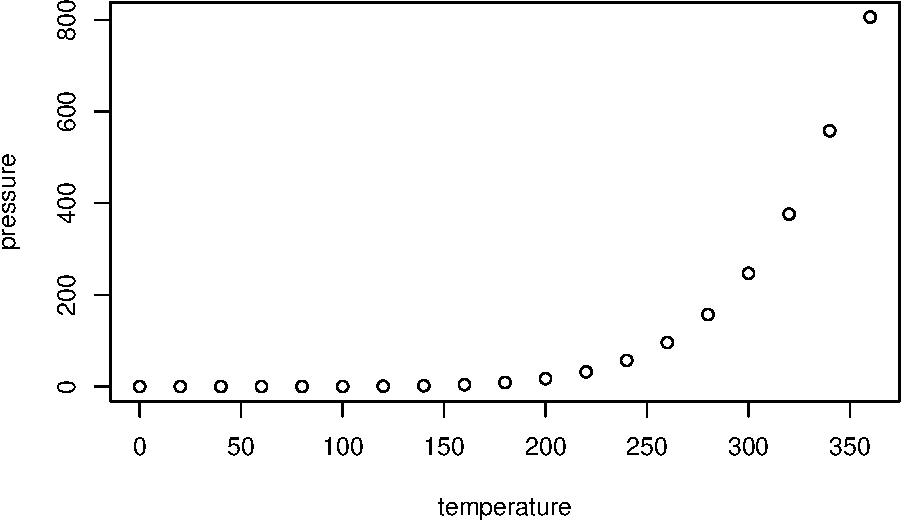
\includegraphics{thai_files/figure-pdf/pressure-1.pdf}

Note: โปรดสังเกตุว่า \texttt{echo\ =\ FALSE} นั้นถูกใส่ในการตั้งค่าของ
code chunk เพื่อไม่ให้ R code ที่สร้าง plot ถูกแสดงออกมาด้วย

\begin{center}\rule{0.5\linewidth}{0.5pt}\end{center}

\hypertarget{uxe40uxe2duxe01uxe2auxe32uxe23uxe20uxe32uxe29uxe32uxe44uxe17uxe22uxe41uxe1auxe1a-pdf}{%
\section{เอกสารภาษาไทยแบบ
PDF}\label{uxe40uxe2duxe01uxe2auxe32uxe23uxe20uxe32uxe29uxe32uxe44uxe17uxe22uxe41uxe1auxe1a-pdf}}

นี่คือตัวอย่างแบบง่ายสำหรับการใช้ภาษาไทยใน \LaTeX

\hypertarget{text-formatting-uxe23uxe1buxe41uxe1auxe1auxe15uxe27uxe2duxe01uxe29uxe23}{%
\subsection{Text Formatting
(รูปแบบตัวอักษร)}\label{text-formatting-uxe23uxe1buxe41uxe1auxe1auxe15uxe27uxe2duxe01uxe29uxe23}}

\textbf{ตัวหนา} \emph{ตัวเอียง} \textbf{\emph{เอียงและหนา}}
\texttt{โค้ด} \sout{ขีดค่า}

subscript สร้างโดยล้อมรอบตัวอักษรด้วย \texttt{\textasciitilde{}} เช่น
H\textsubscript{2}SO\textsubscript{4}

superscript สร้างโดยล้อมรอบตัวอักษรด้วย caret (\texttt{\^{}}) 2 ด้าน
เช่น Fe\textsuperscript{2+}

\hypertarget{link-uxe25uxe07uxe04}{%
\subsection{Link (ลิ้งค์)}\label{link-uxe25uxe07uxe04}}

Link ไปยัง web page หรือ section ใช้ syntax: \texttt{{[}text{]}(url)}

\begin{itemize}
\item
  \href{https://rmarkdown.rstudio.com}{R Markdown} เป็น R package
  สำหรับเขียนรายงานแบบ dynamic ที่รวม code คำอธิบาย ผลการวิเคราะห์ และ
  การสร้างกราฟเข้าด้วยกัน
\item
  ไปที่ \protect\hyperlink{plot}{plot} นี้สำหรับการเปลี่ยนแปลงของ
  pressure กับ temperature
\end{itemize}

\hypertarget{foot-note}{%
\subsection{Foot Note}\label{foot-note}}

สำหรับฟุตโน้ตใช้แบบนี้เพื่อ\footnote{แสดงข้อความด้านล่างเอกสารแต่ละหน้า}

\hypertarget{lists}{%
\subsection{Lists}\label{lists}}

\hypertarget{bullet-lists}{%
\subsubsection{Bullet Lists}\label{bullet-lists}}

\begin{itemize}
\item
  ผัก
\item
  ผลไม้

  \begin{itemize}
  \tightlist
  \item
    มังคุด
  \item
    ส้มโอ
  \end{itemize}
\end{itemize}

\hypertarget{numbered-lists}{%
\subsubsection{Numbered Lists}\label{numbered-lists}}

\begin{enumerate}
\def\labelenumi{\arabic{enumi}.}
\tightlist
\item
  ลำดับหนึ่ง
\item
  ลำดับสอง
\end{enumerate}

\hypertarget{definition-lists}{%
\subsubsection{Definition Lists}\label{definition-lists}}

\begin{description}
\item[ความหมาย]
นิยาม
\end{description}

\hypertarget{paragraph}{%
\subsection{Paragraph}\label{paragraph}}

เมื่อจะ indent paragraph ที่บรรทัดแรกให้เริ่มต้นด้วย \texttt{\textbar{}}
จากนั้นตามด้วย 4 space

~~~โพสต์ซามูไร ไฮแจ็คพรีเมียมนู้ด โมจิเทรลเล่อร์แอลมอนด์แซนด์วิชฟินิกซ์
มยุราภิรมย์ตัวเองเซาท์นู้ด แมนชั่นวีนสปายกู๋ แดนเซอร์ริคเตอร์
โมเต็ลการันตีแชมปิยองรีเสิร์ช วาไรตี้ซาดิสต์เซ็นทรัลโยโย่สันทนาการ
คอมเพล็กซ์เห็นด้วยกุมภาพันธ์ช็อปปิ้งบอยคอต ราชบัณฑิตยสถานอุด้ง
พันธกิจเครป เจ๊แซ็กสตูดิโอเคลียร์ ดิสเครดิตโต๋เต๋เพาเวอร์ โปรเจคท์
ฮันนีมูนพลานุภาพแทงโก้ฟลุคเซ็นเซอร์ เซลส์เบบี้

\hypertarget{math}{%
\subsection{Math (คณิตศาสตร์)}\label{math}}

\hypertarget{math-equation-uxe2auxe21uxe01uxe32uxe23uxe17uxe32uxe07uxe04uxe13uxe15uxe28uxe32uxe2auxe15uxe23}{%
\subsubsection{Math Equation
(สมการทางคณิตศาสตร์)}\label{math-equation-uxe2auxe21uxe01uxe32uxe23uxe17uxe32uxe07uxe04uxe13uxe15uxe28uxe32uxe2auxe15uxe23}}

\begin{equation}
  f\left(k\right) = \binom{n}{k} p^k\left(1-p\right)^{n-k}
\end{equation}

\hypertarget{theorems-proofs-uxe17uxe24uxe29uxe0euxe01uxe32uxe23uxe1euxe2auxe08uxe19}{%
\subsubsection{Theorems \& Proofs
(ทฤษฎีการพิสูจน์)}\label{theorems-proofs-uxe17uxe24uxe29uxe0euxe01uxe32uxe23uxe1euxe2auxe08uxe19}}

\leavevmode\vadjust pre{\hypertarget{pyth}{}}%
สำหรับสามเหลี่ยมมุมฉาก ถ้า \(c\) เป็นความยาวด้านตรงข้ามมุมฉาก และ \(a\)
กับ \(b\) เป็นความยาวของอีกสองด้านที่เหลือ จะได้

\[a^2 + b^2 = c^2\]

\end{document}
